\chapter{USB Subsystem Modifications}
\label{usb-refactoring}

% TODO

\section{Explicit Device Removal}

One of the project goals is to alter the USB subsystem to allow support for
explicit device removal. Such feature can be found in most modern operating
systems and is often used to ensure that devices are left in a consistent state
after a physical port detachment occurs.

The explicit device removal feature usually provides a frontend interface in
the operating system, through which users can observe currently connected
devices and, if needed, issue a signal to the operating system that their
physical detachment is imminent. Following that, the system is expected to
promptly terminate all ongoing communications with the device and signal the
user back. After receiving the confirmation, user can then safely unplug the
device from the system bus without any risk of interrupting communications,
which could otherwise result in undefined state of the device.


\subsection{Considerations}

In the USB protocol, communications between the host and the device take place
in the form of \textit{transfers}. Depending on its version, the host controller
may have various roles in the realization of these transfers. For that reason,
version-specific modifications are carried out separately in host controller
drivers, whereas common functionality is implemented in the bus module, which is
a part of \lib{libusbhost}.

The disconnection routine for explicit device removal is implemented as follows:
~
\begin{enumerate}
	\item The user signals the intention to disconnect a USB device.
	\item The respective device drivers are notified to end their business (e.
		g. flush buffers or close files), possibly scheduling a multitude of
		transfers to the device.
	\item The HC driver disables the capability to schedule new transfers to the
		device.
	\item The HC driver aborts all leftover active transfers to the device.
	\item The device configuration is dropped, leaving it in the
		\state{Addressed} state, in which it is considered safe to be
		physically removed from the bus.
\end{enumerate}

If the user requests that this routine is rolled back, the steps of the
disconnection routine are just executed in reverse order. The following can
therefore be labeled as a reconnection routine:
~
\begin{enumerate}
	\item The user signals the intention to resume communications with a USB
	device, on which the disconnection routine has been previously performed.
	\item The HC driver configures the device.
	\item The HC driver enables the capability to schedule new transfers to the
	device.
	\item The operating system is notified that the device is reachable and
	matches it to appropriate drivers, which initiate communications with it.
\end{enumerate}

The specialization of both routines is performed in the same way as other bus
module interactions. All HC drivers hand off their DDF and device callbacks to
the bus module, which then calls them back to perform low-level commands related
to specific devices, endpoints and transfers. This way, the high-level logic
contained by the bus module essentially follows the listed descriptions above
and the version-specific extensions are resolved in the respective HC driver
implementations.


\subsection{Offline and Online DDF Signal}

The HelenOS Device Driver Framework includes two user-initiated signals
relevant to the implementation of this feature.

\begin{description}
	\item[Offline Signal]
		This signal informs a driver attached to a DDF node that its managed
		device may be removed in the near future. The driver is expected to
		immediately cease all user operations on the device and unbind its
		child DDF functions, possibly sending a \textit{Device Remove} signal
		to all their attached drivers in the process.

	\item[Online Signal]
		This signal is a logical counterpart to the previous signal.
		It informs a driver attached to a DDF node that its managed device will
		not be removed in the near future. The driver is expected to expose all
		child DDF functions related to the device, possibly sending a
		\textit{Device Add} signal to all their matched drivers in the process.
\end{description}

These signals can be easily issued by the user from the system shell by means
of the \app{devctl} application. See Listing \ref{lst:devctl-offline-online}
for invocation example.

\begin{listing}
	\begin{bdsh}
		# Prepare the unplug high speed device at address 2.
		devctl offline /hw/pci0/00:04.0/usb2-hs

		# We changed our mind. Bring the device back online.
		devctl online /hw/pci0/00:04.0/usb2-hs
	\end{bdsh}
	\caption[Example usage of \app{devctl} to issue offline and online
	signal.]{Example usage of the \app{devctl} application to issue offline and
	online signal to a USB high speed device at address 2. The host controller
	PCI address is \texttt{00:04.0}.}
	\label{lst:devctl-offline-online}
\end{listing}

It follows that these signals can be used for the implementation of the
explicit device removal at the level of USB host controller drivers. For that
reason, \lib{libusbhost} has been extended to handle appropriate DDF callbacks
for functions corresponding to HC's child devices. Their handling is forwarded
to the bus module, which executes the disconnection or the reconnection routine
for the \textit{offline} and \textit{online} signal respectively. In addition,
the transfer scheduling mechanism of the bus module has been extended to permit
scheduling new transfers only to devices, which are in the online state.

The general scheme of stopping communication with a device breaks down to
unregistering all its registered endpoints. The biggest challenge the driver
faces is to abort all currently running transfers on an endpoint that is being
unregistered. The majority of transfers (Bulk, Control, Isochronous,
Interrupt-out) wouldn't pose a problem -- we could just wait the short while
until they are completed, either successfully or not. But then there are
Interrupt-in transfers, which, especially in case of gone device, may not
complete in a timely manner.

\subsection{Aborting active transfers}

It is not possible to ``abort a transfer'' in a generic way, mainly because of
synchronization issues. Before we explain how can a transfer be properly
aborted in various Host Controllers, let us describe the lifecycle of
a transfer batch, a structure representing a transfer in HC drivers.

Currently, USB stack in HelenOS only supports synchronous interface to interact
with pipes. The two methods are called \fnc{dev_read} and \fnc{dev_write}.
Driver calls these methods on pipes, and provides a buffer -- either filled
with data, or to be filled. Once the call crosses the IPC barrier, it is joined
to a call to \fnc{bus_device_send_batch}. This function finds the target
endpoint structure, and passes control to \fnc{endpoint_send_batch}.

There, an instance of \struct{usb_transfer_batch_t} structure is created and
filled with parameters of the transfer. It is then passed to the driver
implementation to be scheduled. The driver typically copies the data to
a buffer suitable for the device, prepares some supporting structures, and
finally, schedules the transfer to the hardware.

Since then, an interrupt may come and finish the transfer in a different
fibril. A transfer is finished by copying the data out from the hardware buffer
to the batch buffer, setting the error code and calling a completion callback.
This callbacks answers the original incoming IPC call, causing the \fnc{dev_read/write}
function to return. After that, the transfer batch is destroyed.

But that's not the only scenario that may happen. From the moment a transfer is
created, a pointer to it must not be forgotten, otherwise the caller would
never return. But on the other side, once the pointer to batch is stored
somewhere, the transfer might be aborted at any time. Furthermore, once the
transfer is scheduled to the hardware, the buffers must not be deallocated
until the driver is sure that the hardware won't use them anymore.

This synchronization problem might be resolved by locking the batch and
reference counting, but then different problems would arise (e.g. a transfer
could be finished after the endpoint was successfully unregistered, just
because we cannot know if there's any). So, we decided to take a different
approach.

As the interface is synchronous (and it doesn't make much sense to make it
asynchronous, unless under special conditions), and the endpoint is assumed to
be available for one driver only, there's no point in having more than one
transfer active at a time. So, we store the pointer to a batch inside the
endpoint structure, in the field \struct{active_batch}. This field shall not be
accessed, unless the endpoint guard is locked.

The driver shall modify this field only by calling two methods, which ensure
the proper semantics: \fnc{endpoint_activate_locked} and \fnc{endpoint_deactivate_locked}.
Both of them are to be called with the guard locked. An endpoint is said to be
\emph{active}, if there's an active transfer scheduled. Once the endpoint is
activated and the guard released, the batch must be assumed to be already
finished or aborted. In the counterpart process, when the driver wants to
finish or abort transfer, it needs to obtain the endpoint guard, check if the
transfer is still the active transfer, and then deactivate the endpoint.

In other words, the ownership of the batch is transferred from the calling
fibril to the endpoint once activated, and to the finishing/aborting fibril by
deactivating the endpoint. Only the owner of the batch is allowed to finish it.

Following this scheme a driver can be sure a batch is always finished once and
only once. But in our thoughts, we haven't yet covered that the buffers of the
batch are owned by the Host Controller while the batch is scheduled. Because of
that, drivers need to implement aborting transfers themselves.

The version-specific part of the implementation is discussed in the next sections.


\subsection{UHCI, OHCI and EHCI specifics}

All three HCI's that were supported prior to our project have similar
structure with regard to what is required to implement transfer aborting. Let us
first describe very briefly how these controllers handle transfers.

Generally, all three host controllers require driver to create a system of
linked structures in memory (for UHCI and OHCI, restricted to the lower 4 GBs
of addressable space). The names and guts differ, the structures however
describe a linked chain of queues. Queues are then filled by transfer
descriptors, which describe USB transfers to be done. Once the transfer is
done, its descriptor is flagged, removed from the queue and if the descriptor
is marked, the host is interrupted. More specific information can be found
either in respective specifications, or in the documentation of the HelUSB
project.

At the time of receiving an interrupt, the host does not know which transfer
was finished, so it has to check all pending transfer descriptors for the
completion flag. In case all the transfer descriptors of a transfer are
completed, the driver may finish the transfer.

When aborting a transfer, the driver must make sure the controller is not using
any of the allocated buffers. It is allowed to modify the queues while the
controller is scanning them, the modifications must however follow an order in
which the consistency of the structure is guaranteed at any time. After it
does, it must notify the driver that the structure has changed, in order to
force the controller to clear its caches (EHCI only).

Because the driver is polling the transfers for completion, the first thing
we (as a driver) have to do to abort a transfer is to remove it from the list
of pending transfers. As the list modification is synchronized, we can be sure
no other fibril will ever complete the transfer. After that, we can finish it
ourselves with an error. Note that in this case it is unknown to driver whether
the transfer was completed or not -- but since the driver is unregistering an
endpoint, the device must already be in a state in which it expects removal.

The removal itself is not that easy as one would expect, because it involves
two locks. While scheduling the transfer, we (potentially) need to wait, until
the endpoint is free to be activated, so we need to take the endpoint lock first.
On the other hand, when scanning the pending list, we cannot know the
endpoints, and therefore cannot lock them in advance. The resolution of this
conflict is different in every driver

% TODO: In UHCI, it is currently broken, and it struck me while writing the
% documentation. Too late for me to fix it now, gotta go sleep.

In OHCI and EHCI, transfers have to be prepared with previous transfers in
mind. To avoid the conflict, we changed the list of pending transfers to list
of pending endpoints. The endpoint's reference in this list is counted, and it
is possible to check whether the endpoint takes part in the list. We can remove
it if it is without holding the endpoint lock, and then finish the transfer
without holding the list lock, thus avoiding the ABBA deadlock completely.

From the further perspective, these controllers do not have an internal state
for individual devices and endpoints, so the deconfiguration and its rollback
is an operation on software-state only. As such it is already done completely
by the \lib{libusbhost} library.

\subsection{xHCI Specifics}

Since xHCI is the latest HC interface implementation, a lot more is done by the
hardware for the HC driver in comparison with previous versions. The concept of
xHCI command ring leads to very elegant implementation of the required
functionality on the HC driver part.

For the purpose of aborting active transfers, the xHCI features an explicit
\textit{Stop Endpoint} command, which instructs the HC to abort all transfers
to a specific device endpoint. This command is issued by the HC driver for all
removed device endpoints, which are active at the moment of the request.
Furthermore, device configuration is dropped along with all remaining endpoints
by issuing a \textit{Configure Endpoint} command with the DC (deconfigure)
flag.

Reconnection is quite straightforward and requires only that the HC driver
issues a regular \textit{Configure Endpoint} command in order to transition the
device from the \state{Addressed} state back to the \state{Configured} state.


\subsection{Driver Support}

Since the existing USB drivers were quite incomplete, their implementation has
been extended to add support for explicit device removal. This mostly lead to
novel approaches to deallocation of device-related memory structures, which is
often performed in the \fnc{device_remove()} and \fnc{device_gone()} driver
callbacks.

For instance, a number of drivers required that an implementation of
\fnc{device_remove()} is created in the first place. Quite so often, the
existing implementation of \fnc{device_gone()} has provided a good starting
point, given that both functions have to deal with USB device's demise. The
fundamental difference was that while \fnc{device_gone()} merely dealt with
the fallout of unexpectedly unplugged device, \fnc{device_remove()} had the
opportunity to tie up all lose ends prior to the physical detachment of the
device.

This posed a problem, especially in HID and hub drivers, which heavily relied on
polling of interrupt endpoints. Since polling was a synchronous operation from
the device driver's point of view, a polling fibril has been created when the
driver started managing the device. When the device was unplugged, the polling
operation failed with error, waking up and effectively terminating the fibril in
the process. Since no explicit joining mechanism was available, the
implementation of \fnc{device_gone()} merely spinned a limited number of times,
waiting for the polling fibril to die. This mechanism was however unsuitable for
\fnc{device_remove()}, since the fibril would not awaken due to an error caused
by the physical disconnect, which has not happened yet.

This lead to complete refactoring and extension of the USB device polling
mechanism, which is described in detail in Section \ref{polling-refactoring}.
In summation, the new version of the mechanism allows device drivers to join
their polling fibrils and consistently wake them up in order to avoid deadlocks.

To actually stop the polling in the \fnc{device_remove()} callback, the device
driver has to trigger a transfer abort inside the HC. There's no sensible way
of how to allow a driver abort its own transfer, which wouldn't introduce
potential memory leaks inside HC or synchronization problems. So we decided
that the driver will have to unregister the endpoint as the only way to abort
a currently running transfer (and also disable scheduling of new ones). The
device's endpoints (or, at this layer already called pipes) are completely
managed by the \lib{libusbdev} library. Previously, their lifetime was strictly
tied to the lifetime of the handled device. There are only two possible
ordering of these two operations:

\begin{enumerate}
	\item Close the pipes after the \fnc{device_remove()} callback returns.
		After that, the polling fibrils will end and destroy their structures.
		The library USB device structure will have to be reference-counted and
		the counter will be managed by the driver to account for polling
		fibrils.

	\item Close the pipes prior to calling \fnc{device_remove()}, effectively
		destroying the only reason why this callback exists, and make the
		expected removal equivalent to the unexpected one.
\end{enumerate}

\noindent It is pretty obvious that we had to choose a completely different approach. So
we came up with three more options:

\begin{enumerate}
\setcounter{enumi}{2}
	\item Introduce a new callback, e.g. \fnc{device_removed()}, to be called
		after the pipes are closed. The removal would be split into two phases:
		first, in \fnc{device_remove()} the loose ends are closed and the
		device is brought to a state expecting removal, then in
		\fnc{device_removed()}, the polling fibrils are joined and structures
		are destroyed.

	\item After calling \fnc{device_remove()} and closing the pipes, call
		\fnc{device_gone()}.

	\item Allow the driver to close individual pipes imperatively.
\end{enumerate}

At first, we decided to go with option 3). But it was yet another callback, we
didn't come up with a name that wasn't so similar and yet was clear, and
finally, the \fnc{device_removed()} callback implementations were very similar
to \fnc{device_gone()}.

The option 4) seems reasonable at the first look, but it would create
inconsistency between DDF drivers and USB drivers, which would be very
confusing for developers. \footnote{Actually, some team members think this
behavior shall be present in DDF too, but we didn't open a discussion with
HelenOS developers.}

In the end, the only option left was letting the driver close its own pipes. So
we introduced a new library call \fnc{usb_device_unmap_ep()}, which does
exactly that. The new library polling mechanism closes its pipe automatically,
but this functionality is usable in any driver for any endpoint.

The implementation of explicit device removal support for the rest of the
drivers was a trivial extension of their previous functionality.


\section{Polling Mechanism Improvements}~\label{polling-refactoring}

As hinted by the previous section, the USB device endpoint polling mechanism has
been completely refactored.


\subsection{Before State}

In the original state, USB device drivers had to configure polling using a
configuration structure \struct{usb_device_auto_polling_t}, then pass this
structure to one of four functions:

\begin{itemize}
	\item \fnc{usb_device_auto_poll()},
	\item \fnc{usb_device_auto_poll_desc()},
	\item \fnc{usb_device_auto_polling()},
	\item \fnc{usb_device_auto_polling_desc()}.
\end{itemize}

These functions copied the configuration and started an automated polling
fibril, which interacted with the deice driver using callbacks specified in the
configuration structure. At the end of the polling, the fibril deallocated all
of the resources and terminated.


\subsection{Motivation}

There was a number of problems with the status quo:

\begin{itemize}
	\item The semantics of functions used to initiate polling was not clearly
		distinguished by their name (and neither their documentation).
	\item In addition, the polling functions had a high number of arguments,
		which opened possible room to device driver errors due to their
		misinterpretation (or further API changes in the future).
	\item The polling fibril was detached at the moment of polling start and
		could outlive the device in the driver's memory, then fail later when
		accessing memory, which was already freed in \fnc{device_remove()} or
		\fnc{device_gone()}. Some drivers bypassed this by spinning in these callbacks,
		waiting for the fibril to terminate. However, if the fibril was still
		polling even after a number of attempts, a non-zero error code was returned,
		rendering the entire DDF function (along with its subtree) in a defunct
		state.
	\item The driver was unable to inspect the state of the polling fibril
		directly, so often a flag had to be created and maintained by polling
		callbacks.
	\item A distinct subset of polling parameters were not configurable and were
		hard-assigned their default values inside function implementation. If the
		driver wanted to change any (and not necessarily all) of such parameters, it
		had to specify all the values by itself. Because the constants were
		hard-coded in the implementation, the driver then usually had to copy the
		values.
\end{itemize}


\subsection{Modifications}

\begin{figure}
	\centering
	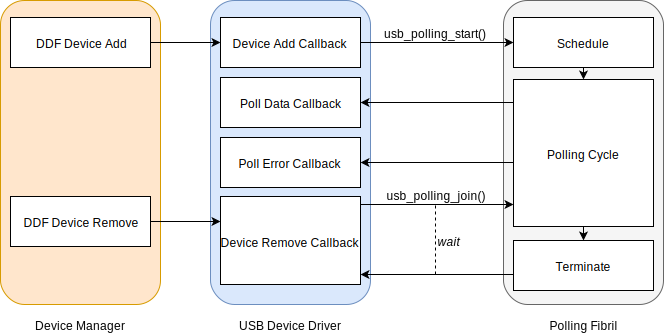
\includegraphics[width=0.8\textwidth]{usb-polling}
	\caption[USB device polling interactions diagram.]{A diagram of interactions
	between the Device Manager, USB device driver and one of its polling fibrils
	during its lifecycle.}
	\label{fig:usb-polling}
\end{figure}

The configuration structure \struct{usb_device_auto_polling_t} has been renamed
for simplicity sake to \struct{usb_polling_t}. Instead of serving as a one-time
configuration structure during polling initiation, its role changed to represent
the entire instance of the polling process throughout its lifetime.

Introducing standard functions such as \fnc{usb_polling_init()} and
\fnc{usb_polling_fini()}, the device driver is now fully responsible for the
ownership of the structure. This is convenient, since drivers often have their
own structures for device data, where \struct{usb_polling_t} can be placed as a
field, dropping the need for additional calls to \fnc{malloc()} and
\fnc{free()}. In addition, this resolves the problem with default values of
various configuration parameters, since in \fnc{usb_polling_init()} all
parameters are assigned their default values and device driver can override only
those desired.

All four of the original polling initialization functions were unified into a
single function \fnc{usb_polling_start()}. Since there is now a clear structure,
which represents the polling instance, the arguments of the original four
functions were moved to \struct{usb_polling_t}, where they are clearly named and
documented, preventing any possible errors from their misinterpretation. Suffice
it to say, that the original four functions mostly fulfilled the role of syntax
sugar, which is now rendered unnecessary, given the fact that default values of
configuration parameters are pre-filled in the polling structure.

Lastly, the API was extended with the \fnc{usb_polling_join()} function, which
closes the polling pipe and consistently waits until the polling fibril
terminates. This function addresses the problem of spinning in driver's
\fnc{device_remove()} or \fnc{device_gone()} callbacks, or possible negligence,
which may result in the polling fibril outliving the device and then accessing
invalid memory. Calling this function in this context will result in the
immediate and synchronous termination of the polling mechanism prior to
deallocation (as depicted in Figure \ref{fig:usb-polling}).

Furthermore, the exposure of internal polling parameters now gives device
drivers more creativity in their approach to polling. For instance, drivers can
now inquire about the state of the polling fibril without the need to have a
private flag maintained by their polling callbacks. The drivers can also change
polling parameters such as request size or polling delay mid-flight, which is a
more flexible approach than to stop polling, change parameters and then start
polling again (note that stopping polling at will was not supported by the
previous implementation without generating actual errors from the hardware
device).

A nice minimalist example of the new polling mechanism usage can be found in
Listing \ref{lst:polling-example}

\begin{listing}
	\begin{code}
		static usb_polling_t polling;
		static uint8_t buffer[13];

		static bool callback(usb_device_t *dev, uint8_t *buffer, size_t size, void *arg)
		{
			printf("Have data!/n");

			// Return true if we wish to continue polling.
			return true;
		}

		static void demo()
		{
			// Initialize.
			usb_polling_init(&polling);

			// Configure.
			polling.device = /* some usb_device_t here */;
			polling.ep_mapping = /* some interrupt(in) endpoint of the device */;
			polling.buffer = buffer;
			polling.request_size = sizeof(buffer);
			polling.on_data = callback;

			// Start polling.
			usb_polling_start(&polling);

			// Sleep synchronously for a while.
			async_usleep(10000);

			// End polling and clean up.
			usb_polling_join(&polling);
			usb_polling_fini(&polling);
		}
	\end{code}
	\caption{Minimal usage example of the new USB device polling mechanism.}
	\label{lst:polling-example}
\end{listing}



\section{A Library Module for USB Hubs}
\label{hub-port-refactoring}

We introduced a new module to support writing hub drivers:
\file{uspace/lib/usb/include/usb/port.h}{usb/port.h}. It solves the problem of
hub drivers, that events are announced through a single channel, even though
they need to wait for each other. The implementation of this module was
motivated not only by the need of refactoring, nor because we wanted to share
the functionality with the xHCI driver, but because the previous implementation
of \lib{usbhub} driver synchronized the fibrils wrong. There might have been
situations in which two fibrils were spawned and enumerated the same device.

To solve the issue a state information is managed for every port, represented
by the structure \struct{usb_port_t}. It contains the current port state, one
of the following:

\begin{description}
\begingroup \leftskip=1cm \rightskip=\leftskip
\setcounter{enumi}{-1}
	\item[\state{Disabled}]
		There has been no activity on the port yet, or it is already over.
		Initial state.

	\item[\state{Connecting}]
		A connected event came, the enumerating fibril was started. It hasn't
		finished yet, so the device is not enumerated yet. Also, the device is
		still connected, no error event came while the connecting is in
		progress.

	\item[\state{Enumerated}]
		The device was successfully enumerated, so it has to be removed after
		it will be disconnected.

	\item[\state{Disconnecting}]
		A disconnected event came after the device was enumerated, so
		a removing fibril was started.

	\item[\state{Error}]
		An event about the device disconnection state came while the
		enumeration was in progress, so the enumeration fibril has to be
		stopped. This is achieved by returning \macro{EINTR} from the waiting
		methods.

\endgroup
\end{description}

The basic synchronization invariant is that the state never changes unless the
guard is locked. It is expected that the guard is not held for a long time, so
the fibril generating events shall not be blocked indefinitely. The only
exception being the final phase of enumeration (announcing the device to the
bus), which once started, cannot be easily interrupted -- but this operation on
the bus is also expected to run for a limited time only.

The scheme of states and allowed transitions can be seen on figure
\ref{fig:port-states}.

\begin{figure}[h]
	\centering
	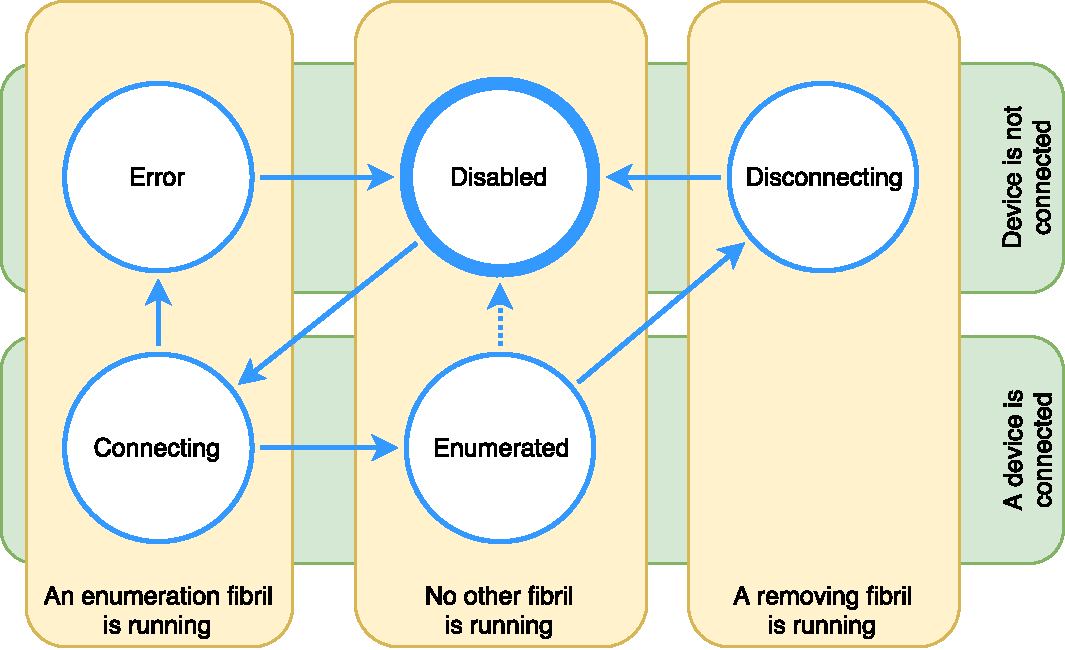
\includegraphics[width=0.6\textwidth]{port-states}
	\caption{A graph of port states and their transitions.}
	\label{fig:port-states}
\end{figure}

The transitions are triggered by delivering events to the module. This is done
by calling following functions:

\begin{itemize}
	\item \fnc{usb_port_connected}
	\item \fnc{usb_port_disabled}
	\item \fnc{usb_port_enabled}
\end{itemize}

The \fnc{connected} and \fnc{disabled} functions take a callback as an
argument. If the respective state transition is triggered, this callback is run
in a separate fibril. These functions can block to obtain the port guard, and
the \fnc{disabled} event can furthermore block while waiting for the
enumeration fibril to terminate. But before it does, it makes sure the worker
will be notified as soon as possible.

To make it work, the callbacks must not block while holding the guard. They
can, however, wait for the enabled event, signalling the completion of port
reset, using a function \fnc{usb_port_wait_for_enabled}. The caller is required
to check the return value of it -- it can either finish with \macro{EOK},
timeout with \macro{ETIMEOUT} or be interrupted with \macro{EINTR}. The enabled
event is sent by calling the function \fnc{usb_port_enabled}.

When this fibril management is separated, an implementation of USB hub driver or
root hub driver is very simple. The hub driver just initializes the
\struct{usb_port_t} structure for every port it manages, then waits for events
from the hardware (either by poling the \textit{Status Change Endpoint}, or by
waiting for an interrupt), and forwards the events to this module, providing an
implementation of the enumeration and removal process.

One last thing to note is what to do when the structure is finalized, but
a device is still connected. It might happen that there is a subtree of devices
and hubs being removed because the subtree root $R$ has been unexpectedly
removed. In that case, a port disconnect is delivered to the parenting hub,
which triggers the device removal process. The hub $R$ then receives the DDF
signal \fnc{device_offline}, and starts removal if his own children. But
there's a catch: USB hierarchy is presented as a flat one to the DDF framework.
That means that the devman has no clue about hubs (it sees them as ordinary USB
devices), and considers that all of them are connected to the HC directly.
Device removal is prepared for the situation that device will remove also its
\textit{children} devices, but serializes removal of \textit{sibling} devices.
Therefore, recursive removal of hubs creates a deadlock in devman.

Fortunately, the HC driver must be prepared for badly written drivers, so it
cleans up after the device function is unbound. This cleanup includes also
removal of its former children devices -- so the workaround for this problem is
simply leaving those devices connected, as the HC will remove them itself. This
state transition is denoted by dotted line in the graph, and is triggered by
finalizing the port structure while a device is enumerated.

\section{USB Tablet Driver}

This modification is very standalone and seemingly simple, yet very useful and
appreciated. We extended the HID driver to support absolutely positioned
devices. That means, one can now connect a USB tablet and it will work in
HelenOS. If you are still wondering what this could be useful for (people using
USB tablets are usually graphic designers or photographers, not microkernel
developers), try running QEMU with an emulated one:

\begin{bdsh}
$ qemu-system-x86_64 -enable-kvm -usb -device usb-tablet -boot d -cdrom image.iso
\end{bdsh}

When using mouse with relative positioning (PS/2, USB mouse), one has to first
click inside the window of QEMU to let it grab input. To release it again,
a special key combination (for current QEMU Ctrl+Alt+G) must be pressed. When
using an emulated USB tablet instead, the mouse is not ``locked'' inside the
window, but it can freely move in and out and still be registered by the guest
OS.

\section{DMA buffers}

A simple but repeated scenario gave rise to another new submodule of
\lib{libusbhost}. It is a very thin abstraction, yet has been proven useful and we
think it could be adopted to \lib{libdrv}, for example.

A common task for drivers is allocating memory for buffers, that are accessible
for DMA. Often there are some restrictions given by the hardware driven -- the
buffer must be placed in the lower 32bit addressable space, it has to be
aligned, physically contiguous, or possibly not crossing a page boundary.

Even if the buffer is intended for the hardware use only (like xHCI
scratchpads), the driver must keep the pointer to where the buffer is mapped
inside its virtual address space in order to release the memory once it is not
needed anymore. Hardware devices do not share the virtual address space with
the task though, so the driver must always obtain also the physical address of
the buffer. To satisfy all of these requirements, the HelenOS kernel offers
a specialized API. The driver just needs to call a function
\fnc{dma_map_anonymous}, and is given both the virtual and physical address. It
is able to specify its requirements using flags. This API is powerful, but
complex and inconvenient to use.

The authors of the former USB stack addressed the complexity by creating
utility functions in \header|<usb/host/utils/malloc32.h>|. These functions offer
a familiar interface of \fnc{malloc}/\fnc{free}. The \fnc{malloc32} function
intentionally discards the physical address provided by
\fnc{dma_map_anonymous}, in order to be simple to use. To retrieve the physical
address later, one can use another utility function, \fnc{addr_to_phys}. This
one is a simple wrapper for a syscall.

Even previous authors of the USB subsystem were aware of it being a syscall,
and tried to cache the physical address where it would be used unneccessarily
multiple times. The usage scheme of these functions then grew wild: the memory
was allocated by \fnc{malloc32}, just to be translated by \fnc{addr_to_phys} on
the next line. These two pointers were then stored inside the same structure.

Being aware of this use-case, we created a different submodule for allocation
of DMA buffers. Instead of a plain pointer, the caller uses a structure called
\struct{dma_buffer_t}. This structure can store both the virtual and physical
address of the buffer, accessible through fields \struct{virt} and
\struct{phys}. The buffer allocation is made simply by using a function called
\fnc{dma_buffer_alloc}, which fills the specified buffer with pointers to
a properly sized allocated space. When the buffer is no longer needed, it is
freed by calling \fnc{dma_buffer_free}.

When the buffer is contiguous in memory, it's easy to calculate the physical
address ourselves, without a help of the kernel. To obtain a physical address
for a concrete position in the buffer, one just needs to call
\fnc{dma_buffer_phys}, which translates a virtual address pointing inside
a buffer to a corresponding physical address.

So far, DMA buffers always assume the strictest requirements for the allocated
memory. That is, the returned memory is page-aligned, physically contiguous,
always in the 32bit addressable space. Should there be a need to loosen one the
constraints (e.g. to reduce the memory footprint), the allocation routine can
be supplied a policy, defining the requirements. There is also a particular
future optimization, for which the mechanism is prepared. Especially the former
HC drivers often allocate a whole buffer, which must be at least
\macro{PAGE_SIZE} big, just to hold a few-bytes sized descriptor structure.
Shall the wasted memory be a problem, one can easily extend this module to use
an allocator in userspace to back DMA buffers.

One more reason to drop the previous \fnc{malloc32} helpers completely is that
developers that are beginners to HelenOS might see \fnc{malloc32} as a weird
name for an ordinary \fnc{malloc}, and start using it to allocate ordinary
memory, which is very wasteful and expensive.
